%% rngs
%% ECE 541 Project 2
%% Kashev Dalmia - dalmia3
%% David Huang   - huang157

\documentclass[conference,11pt]{IEEEtran}

\usepackage[cmex10]{amsmath} % Math
\usepackage{graphicx}        % Images
\usepackage{listings}        % Code Snippets

% 1.3 for 1.5 Line Spacing, 1.6 for Double Line Spacing
\linespread{1.3}

% For URLs
\usepackage[hidelinks]{hyperref}

\begin{document}

\title{Random Number Generators: Implementation and Statistical Analysis Using Dieharder}

\author{\IEEEauthorblockN{Kashev Dalmia}
\IEEEauthorblockA{Email: dalmia3@illinois.edu}
\and
\IEEEauthorblockN{David Huang}
\IEEEauthorblockA{Email: huang157@illinois.edu}
\and
\IEEEauthorblockN{William H. Sanders}
\IEEEauthorblockA{Email: whs@illinois.edu}}

\maketitle
% Force Page Numbers
\thispagestyle{plain}
\pagestyle{plain}

\begin{abstract}
We implement in efficient C++ several kinds of different modern pseudo-random number generators, or PRNGs; a Linear Congruential Generator, a Lagged Fibonacci Generator, an Xorshift type generator, a Complementary Multiply with Carry Generator, and a Mersenne Twister Generator. We discuss the challenges in testing these kinds of PRNGs, and discuss one of the more common frameworks for testing these random number generators. Finally, we compare our results to what we expect from these implementations, as well as comment on the suitability of these PRNGs for use in simulation of systems.

\end{abstract}

\begin{IEEEkeywords}
Random Number Generators, Psuedo Random Number Generators, PRNGs, Statistical Analysis, Dieharder
\end{IEEEkeywords}
\section{Introduction}
\label{sec:introduction}
The applications of randomness are far reaching. From statistics, to simulation, to gaming, to cryptography, there is a large need for random number generators. Oftentimes, these generators must be fast to keep up with the demand produced by high speed applications, such as those used on modern servers to ensure proper security. It is also desirable that they be deterministic in some cases in order to produce reproducable and debuggable simulations. Thus, the creation of pseudo random number generators, or PRNGs, has become an important research area in modeling, computer simulation, and mathematics communities.

In the field of analysis of computing systems, simulation is an extremely important part of the modeling process. Today's stochastic models are so complex that finding analytic solutions is effectively impossible. As such, simulations driven by randomness allow a far more viable way to study the behavior of systems. This is the sort of need that motivates this project: a study of the theory behind random number generators, how to test them, and their suitability for this purpose.

\subsection{Kinds of Random Number Generators}
For the purposes of this paper, there are two kinds of Random Number Generators, or RNGs: Hardware RNGs, and Software RNGs. Hardware RNGs are used not only to output a random bit stream faster than a multipurpose CPU might be able to \cite{Saiprasert:2010:OHA:1857927.1857929,Barel:1983:FHR:800042.801454}, but also in order to gather entropy in a more unpredictable way, such as measuring thermal noise, detecting air moisture, or using unpredictable user interactions, such as keystrokes and mouse motion , to name a few. Often hardware RNGs are used to seed software RNGs. Readers interested in the seeding of RNGs with external entropy are encouraged to read \cite{Hennebert:2013:EHP:2462096.2462122}.

Software RNGs, even when they draw upon these sources of entropy from nature for seeds, are in fact PRNGs, because the software that generates these sequences must be deterministic. In this paper, the term RNG will refer to software PRNGs, unless otherwise indicated. These software RNGs use mathematical models to take a finite amount of state and turn this into a sequence of seemingly infinite random output, suitable for use in a variety of purposes. Though special purpose hardware RNG circuits may be fast, software RNGs are usually faster than repeatedly polling a sensor to gain outside entropy. They are also far more convenient to use, as all is required is a computer, rather than special purpose hardware.

Finally, there are several classes of software RNG based on quality of output. The highest class is those which are suited for cryptography. Generally, this includes passing the next bit test: that if $k$ bits of a random sequence are known, then no polynomial time complexity algorithm should be able to guess the next bit \cite{Yao_1982}. On a similar vein, the previous bits of a random sequence must also be impossible to guess in polynomial time as this would expose the initial state of the generator, and thus the seed. These cryptographically secure random number generators tend to be slow and are not designed to be run more than a few times in quick succession, which makes them unsuitable for use in applications in which speed is necessary, like simulation or Monte Carlo analysis.

This paper deals with RNGs which are not of cryptographic quality, but are nonetheless useful. These RNGs combine speed with memory complexity and quality of output.

\subsection{This Project}
In this project, we study and implement a few common random number generators in C++, from those which have been used historically, to those which are most commonly in use today. We test our generators using the Dieharder test suite \cite{dieharder_website}. Using Dieharder, we can push these RNGs to the point of failure, and therein see their flaws and sutability for various applications. We can also compare our results with the results of the RNGs built into the GNU Scientific Library, or GSL, and thus Dieharder. All of the software written for this project is available on Github \cite{github_repo}.

In this paper, we first discuss the methods and challenges of testing random numbers in Section~\ref{sec:testing}. Then, we discussed the different classes of RNGs we study in Section~\ref{sec:classes}. Finally, we describe our software approach in Section~\ref{sec:software} and share our results in Section~\ref{sec:results}.


\section{Testing Random Number Generators}
\label{sec:testing}
\newcommand{\pvalue}{$p$-value}

Testing random number generators can be tricky. An ideal random number generator can be considered to be independently, identically distributed samples of a uniform distribution $U(0,1)$. However, the RNGs that we consider here are not truly random. So, the crux of the problem is how to determine what set of numbers appear random enough, such that they are suitable for use.

\subsection{The Empirical Approach}
\label{sec:empirical}

Imagine flipping a coin 10 times and recording the number of heads and tails. For a fair coin, one would expect to get roughly the same number of heads and tails. If one got 10 heads, and only 1 tails, one might be inclined to suspect that this coin might not be a fair and truly random coin. However, this event has a distinct nonzero probability of this happening, described by the pdf of the binomial distribution:
$$ \binom{10}{9} \frac{1}{2}^{9} \frac{1}{2} = 0.00977$$
In other words, even for a fair coin, in 1000 trials of 10 coin flips, one would expect to get 9 heads and 1 tails 9 or 10 times. Similarly, imagine if one had a different coin, and ran this same test, but always got exactly 5 heads and 5 tails, for all 1000 trials. Though on average we expect to get about the same number of heads and tails, this coin is also suspect, because for all these repeated trials, we should expect them to follow the binomial distribution discussed above.

If we increased the number of flips per trial to a very large $n$, and increased the number of trials to a very large $t$, the expected distribution should appear increasingly similar to the normal distribution, with mean heads percentage of $\mu = 0.5$. This is verified by the Central Limit Theorem \cite{central_limit_theorem}.

So taking again our mystery coin, if we apply the test with reasonably sized $n$ and $t$, and get a distribution of our sample means, we expect it to resemble a normal distribution but will likely not be perfect. There is a certain probability, if we assume that the underlying RNG is perfect, that the result we got would occur: a number on the range $(0,1)$. We shall call this our \pvalue. If this \pvalue~is very, very small (on the order of $10^{-6}$), we might say with a certain degree of confidence that our assumption that the RNG is good is incorrect. However, we could be more confident if we repeated this process several times, and looked at the distribution of \pvalue s.

We can find the probability of getting our \pvalue~distribution using a Kolmogorov-Smirnov test \cite{}, which quantifies the difference between the expected distribution and the \pvalue distribution that we observe. This test yields a second \pvalue: the probability that the resultant distribution would occur given that the underlying RNG is indeed indistinguishable from a perfect one.

If this second \pvalue~is low, then we can safely decide that the RNG being tested is not good. In other words, statistically speaking, the underlying RNG is differs from a perfect RNG by a significant amount. If this value is high, then, rather than accept that the RNG is `good', we instead conclude that we cannot reject our hypothesis that it is `good'.

In fact, this process is exactly what the Dieharder test suite does, and interested readers are encouraged to see \cite{dieharder_manual} for further information. Our implementations of RNGs are used to pipe random numbers to Dieharder, which does this sort of analysis for several different kinds of tests, which are discussed next in Section~\ref{sec:dieharder}

\subsection{Dieharder}
\label{sec:dieharder}

Dieharder's man page states that ``[...]dieharder can eventually contain all rng tests that prove useful in one place[...]'' \cite{dieharder_website}. It aims to be a one-stop-shop for testing RNGs. It is the spiritual successor and improvement to George Marsagalia's Diehard testing tool, which in turn is a testing tool which took many tests from the famous Donald Knuth \cite{diehard}. Though it is not the only set of tests or testing suite of this kind \cite{donald1999art,diehard,nisttoolkit,L'Ecuyer:2007:TCL:1268776.1268777}, it holds the distinction of being readily available in the Ubuntu package repository, and having good documentation \cite{dieharder_manual}.

Dieharder has many tests, listed in Table~\ref{tab:diehard_tests}. It is worth discussing a few of the tests available in Dieharder to give the reader an idea of what sort of things are tested, and furthermore, what failing one of these tests might indicated about the quality of an RNG. Further information about tests not discussed is available in the Dieharder man pages and help flags.

\begin{table}[tb]
  \caption{Available tests in Dieharder version 3.31.1.}
  \label{tab:diehard_tests}
  \begin{center}
    \begin{tabular}{l | l | l}
    \hline
    \hline
    \textbf{\#} & \textbf{Test Name} & \textbf{Reliability} \\
    \hline
0   &                      Diehard Birthdays  &        Good \\
1   &                         Diehard OPERM5  &        Good \\
2   &              Diehard 32x32 Binary Rank  &        Good \\
3   &                Diehard 6x8 Binary Rank  &        Good \\
4   &                      Diehard Bitstream  &        Good \\
5   &                                Diehard OPSO  &     Suspect \\
6   &                           Diehard OQSO  &     Suspect \\
7   &                            Diehard DNA  &     Suspect \\
8   &          Diehard Count the 1s (stream)  &        Good \\
9   &            Diehard Count the 1s (byte)  &        Good \\
10  &                    Diehard Parking Lot  &        Good \\
11  &    Diehard Minimum Distance (2d Circle) &        Good \\
12  &    Diehard 3d Sphere (Minimum Distance) &        Good \\
13  &                        Diehard Squeeze  &        Good \\
14  &                           Diehard Sums  &  Don't Use \\
15  &                           Diehard Runs  &        Good \\
16  &                          Diehard Craps  &        Good \\
17  &                Marsaglia and Tsang GCD  &        Good \\
100 &                            STS Monobit  &        Good \\
101 &                               STS Runs  &        Good \\
102 &               STS Serial (Generalize)  &        Good \\
200 &                   RGB Bit Distribution  &        Good \\
201 &       RGB Generalized Minimum Distance  &        Good \\
202 &                       RGB Permutations  &        Good \\
203 &                         RGB Lagged Sum  &        Good \\
204 &            RGB Kolmogorov-Smirnov  &        Good \\
205 &                           Byte Distribution  &        Good \\
206 &                                     DAB DCT  &        Good \\
207 &                          DAB Fill Tree  &        Good \\
208 &                        DAB Fill Tree 2  &        Good \\
209 &                          DAB Monobit 2  &        Good \\
    \hline
    \hline
    \end{tabular}
  \end{center}
\end{table}







\subsubsection{The STS Monobit Test}
Taken from the NIST Statistical Test Suite \cite{nisttoolkit}, this test is exactly the test described above in Section~\ref{sec:empirical}. The number of ones are counted in a bit stream generated by a random number generator, and the same analysis is done on it. It is not an extremely rigorous test; some bad RNGs will still pass it but this test is good at weeding out extremely poor RNGs.

\subsubsection{The Diehard Birthdays Test}
Taken from Diehard, the Birthdays Test is so named for the Birthday Paradox: That in some set of $n$ randomly chosen people in a room, the probability that two of them share the same birthday becomes high astonishingly quickly, reaching $99.9\%$ at $n=70$ \cite{abramson1970more}, assuming the distribution of birthdays is uniform. If these birthdays are placed in a year then the distance between pairs birthdays should follow a Poisson distribution. The test in Dieharder places 512 birthdays in a 24 bit `year' and determines if the the resultant distribution is in fact Poisson using the \pvalue~analysis described above.

\subsubsection{RGB Lagged Sums}
Written by the main Dieharder author Robert G. Brown, this test is the only test in the Dieharder suite which tests for lagged correlations. Imagine that, overall, an RNG's output seemed very random, but every seven bits, the same pattern emerged throughout the generation. This test checks for that situation, with several different lag numbers, when running all tests. The lagged bits are taken, used to create single precision numbers between 0 and 1, then $t$ of these numbers are summed. A single trial should have a mean $\mu = 0.5 t$. Then, the \pvalue s are determined from several trials of $t$ sample sums. Interested readers are encouraged to see \cite{dieharder_manual} for a more discussion.

\subsection{Interpreting Dieharder Results}
The authors of Dieharder are careful to avoid saying that Dieharder can verify that a random number generator appears truly random. Rather, Dieharder serves as a set of tests which can weed out poor RNGs, and say with certainty that they do not appear truly random under scrutiny. This is not to say that they are not useful; for instance, if one is simply creating a website which provides a virtual die for a user to roll, then the RNG powering the die need not necessarily pass every Dieharder test (perhaps only the Diehard Craps Test, which specifically tests using an RNG to power dice for a game), but rather pass a majority of them, and still fulfill the requirements. However, if one is running Monte Carlo simulations, an RNG of a higher quality may be desired, which passes more tests.

A system designer must take into account the trade offs between quality of RNG output, memory efficiency, speed, and complexity of implementation when choosing an RNG for a system. These days, with computers as fast as they are, and many programming languages having already chosen a de facto RNG, this choice is hidden from most users, but is still relevant to mathematicians, those who work with large simulations, or others concerned with extremely high quality of randomness and speed.

What does failing a Dieharder test look like? We look back to the \pvalue~analysis; This final \pvalue~represents the probability that, given that the underlying PRNG resembles a true RNG, the series of our tests would yeild the results that they did. The final \pvalue~is a probability on the range $(0,1)$. If this probability is extremely low or extremely high, then the result is considered to be a test failure.

In Dieharder specifically, if the \pvalue~$p$ is $p > \%99.95$ or $p < \%0.05$, then the test is regarded as failed, which is an extremely high threshold. If $p > \%99.5$ or $p < \%0.5$, then the test is marked as weak performance on the part of the RNG. In either the case of the failure or weakness result, it may be worth re-running the test using a different seed to see if this result is consistent. After all, there is some degree of randomness involved, and finding an area of zero ambiguity is nigh impossible.

\subsection{The Theoretical Approach}
\label{sec:theoretical}

Apart from the empirical approach described above and used in Dieharder, there is also theoretical analysis that can be done with a priori knowledge of the RNG's implementation. For instance, the period of an RNG can be time consuming and memory inefficient to measure empirically, but with knowledge of the generating algorithm, these can be deduced. Additionally some RNG algorithms (specifically the Linear Congruential Generator discussed in Section~\ref{sec:lcg}) have a property where their output falls in planes which can be determined easily, if one knows where to look.

This sort of analysis exposes flaws of specific generator algorithms, but doesn't always provide an even footing on which to analyze the RNGs. The periods of the generators are discussed in each RNG class's section, along with other strengths and weaknesses, but the focus of our project is on the performance of these RNGs in Dieharder.


\section{Classes of Random Number Generators}
\label{sec:classes}
Here we describe a few different kinds of random number generators, the math that makes them work, give examples of each kind, and give their strengths and weaknesses.

\subsection{Linear Congruential Generators}
\label{sec:lcg}
The Linear Congruential class of RNGs, or LCG for short, is a very old and relatively simple random number generator. They are based on the formula for a line, modulo another number. The following recurrence relation defines the LCG.
\begin{equation} \label{eq:lcg}
    X_{n+1} = (aX_n + c) \mod m
\end{equation}
Where the parameters are chosen with the following restraints:
\begin{align*}
    m,   \qquad & 0 < m \\
    a,   \qquad & 0 < a < m \\
    c,   \qquad & 0 \leq c < m \\
    X_0, \qquad & 0 \leq X_0 < m
\end{align*}
If $c = 0$, this particular class of of RNG is called a Lehmer, or Park-Miller RNG \cite{Payne:1969:CLP:362848.362860,Park:1988:RNG:63039.63042}.

The period of such generators depends heavily on the chosen parameters. It can be at most $m$, and as a result, $m$ is often chosen to be the largest number which can fit in the number of bits of the output; usually $2^{32}$ or $2^{64}$. Some common parameter sets in use include MINSTD, and glibc. A set of parameters notoriously deemed unfit for use is called RANDU, and is discussed below. Values for these parameters can be found in Table~\ref{tab:lcg_params}.

\begin{table}[tb]
    \caption{Table of common LCG parameters.}
    \label{tab:lcg_params}
    \begin{center}
        \begin{tabular}{l|ccc}
        \hline
        \hline
        \textbf{Name} & $m$ & $a$ & $c$ \\
        \hline
            MINSTD & $2^{32} - 1$ & 48271 & 0 \\
            glibc & $2^{31}$ & 1103515245 & 12345 \\
            RANDU & $2^{31}$ & 65539 & 0 \\
        \hline
        \hline
        \end{tabular}
    \end{center}
\end{table}

\subsubsection{Strengths}
LCG generators are tiny. They store a single word of state, are easy to seed, and with proper parameter choosing can be quite effective RNGs. However, some of the flaws greatly outweigh the lightweight and speed benefits of LCGs for all but the most basic of platforms, discussed next.

\subsubsection{Weaknesses}

LCGs have a fatal flaw, that is amplified by bad parameter choosing: their outputs fall in easily identifiable planes, as proved by Marsaglia \cite{randomnumbersinplanes}. This is most easily demonstrated by viewing the output of a notoriously bad set of parameters: RANDU. In Figure~\ref{fig:randu_fig}, the output of RANDU is treated as $(x,y,z)$ pairs as it is generated, then these points are plotted. It is obvious that all of the output falls in the same set of planes, and is not even an approximation of a truly random number generator. Better parameter choices alleviate this phenomenon by adding the number of planes that would come up in a test like this, and making them closer together, but the basic problem is unavoidable.

Another issue is the period length; at most the period length is $m$, which cannot be easily increased without increasing the number of bits in the word being operated on, which is not practical on modern architectures. In fact, experts recommend not even considering generators with periods $<2^{50}$ for anything but the most trivial uses \cite{L'Ecuyer:1992:TRN:167293.167354}.

\begin{figure}[tb]
    \begin{center}
        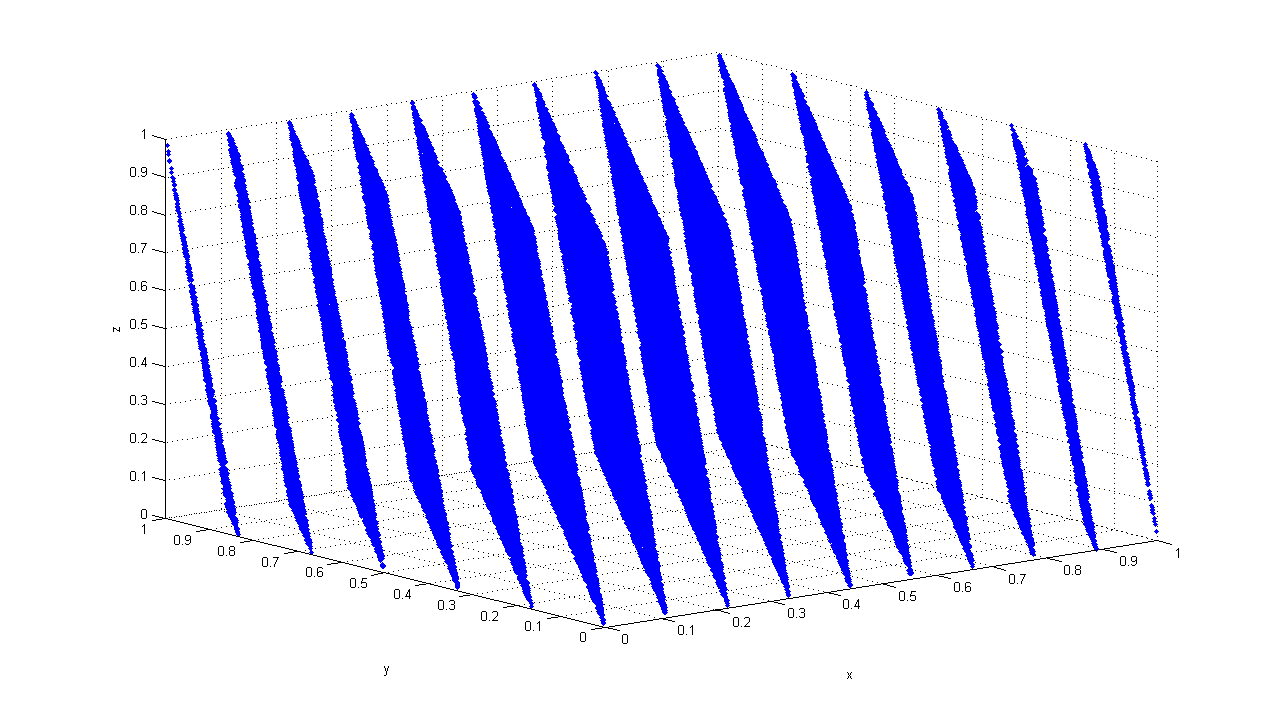
\includegraphics[width=\linewidth]{figures/randu.png}
    \end{center}
    \caption{The problem with LCGs demonstrated by RANDU; a MATLAB plot of consecutive outputs from RANDU used as $(x,y,z)$ points and plotted \cite{randu_fig}.}
    \label{fig:randu_fig}
\end{figure}

Despite these flaws, these extremely small and fast RNGs may still be suited to small embedded architectures and applications where speed is significantly more important than quality.


\subsection{Xorshift Generators}
\label{sec:xorshift}
A far more attractive choice than LCGs for those trying to implement RNGs with a lot of memory constraints, speed requirements, or a combination of the two on an embedded platform, is the Xorshift generator. Discovered and described by George Marsaglia \cite{marsaglia2003xorshift}, they are significantly more adept at creating sufficiently long periods for more applications.

Xorshift RNGs work by keeping a small amount of state (in many example implementations, four numbers), then repeatedly XORing these numbers with shifted versions of themselves. By doing this, the period of the generation can be $2^{32 * 4} = 2^{128}$ with very little code. The following is a short example for how easily Xorshift generators can be implemented. Let \texttt{t}, \texttt{x}, \texttt{y}, and \texttt{w} be seed values. Then, let \texttt{a}, \texttt{b}, and \texttt{c} be the parameters of the RNG. Then, the C style code is as simple as the following:

\begin{lstlisting}[frame=single,language=C++,basicstyle=\ttfamily]
// Random seed numbers
uint32_t t, x, y, w;
// Fixed constants for shifting
const uint32_t a, b, c;
uint32_t get_rand(void){
    t = x ^ (x << a);
    x = y;
    y = z;
    z = w;
    w = w ^ (x >> b) ^ t ^ t( >> c);
    return w;
}
\end{lstlisting}

Picking parameters for the directions and amounts to shift each state variable by is also relatively easy, and is discussed in \cite{marsaglia2003xorshift}, along with every set of appropriate parameters $a$, $b$, and $c$ for 32 bit and 64 bit words.

\subsubsection{Strengths}

Xorshift RNGs are very fast on modern architectures, and use very little state. They have longer periods than LCGs, and are easier to choose parameters for. These RNGs also perform far better on the Dieharder tests than LCGs, and pass the majority of them rather convincingly.

\subsubsection{Weaknesses}

However, the periods of Xorshift generators are not as large as some other generators. They are suitable for most uses, but in large simulations and Monte Carlo analysis, where massive amounts of random numbers are needed, the relatively small period could affect results.


\subsection{Lagged Fibonacci Generators}
\label{sec:laggedfib}
This section will describe Lagged Fib Generators.
\url{http://en.wikipedia.org/wiki/Lagged_Fibonacci_generator}
Also Mention Subtract with Carry:
\url{http://en.wikipedia.org/wiki/Subtract_with_carry}


\subsection{Multiply With Carry Generators}
\label{sec:mwc}
\def\lc{\left\lfloor}   
\def\rc{\right\rfloor}

Multiply With Carry generators, or MWCs are very similar to the previously discussed LCG generators. The primary difference is that rather than adding a constant $c$ during each operation, a value is carried over and added from the previous operation. The concept of variable lag as a parameter is also borrowed from Lagged Fibonacci generators. This givens MWCs the general form:
\begin{equation} \label{eq:mwc}
    X_{n+1} = (aX_{n-r} + c_n) \mod m
\end{equation}
Where $c_n$ is given by:
\begin{equation} \label{eq:mwc_c}
    c_n = \lc \frac{aX_{n-1-r} + c_{n-1}}{m} \rc
\end{equation}
The value of $c_n$ is simply the `carry' or overflow from the previous operation.

The combination of variable lag and nonconstant addends allow MWC generators to have much longer periods than their LCG counterparts as well as greater randomness. Intuitively, this is due to the storage of additional data about the prior sequence. In LCG generators, the amount of overflow from each operation is simply discarded via the modulo operation. Here, that overflow is stored and used as part of the internal state.

\subsubsection{Strengths}
Built on the very lightweight LCG generator, MWC generators share the desirable property of being very fast, as it is computed using a small number of basic arithmetic operations. The addition of the carried term greatly increases the period of this type of generator, up to nearly $m^2$ in some cases.

\subsubsection{Weaknesses}
Just like other generators utilizing lag, MWC generators require additional memory to store its state compared to LCG generators, making it slightly less desirable when used in memory-constrained applications. Also like other lagged generators, seeding a MWC generator may require some finesse not needed in seeding the LCG generator.


\subsection{Mersenne Twister Generators}
\label{sec:mt}
One of the most commonly used RNGs, the Mersenne Twister (MT), was originally discovered by [?]. It is essentially an extension on top of the classical linear feedback shift register (LFSR). A simple LFSR is comprised of a bitwise shift-register where its input is determined by some combination of its current contents, traditionally the XOR of a select few bits from the register. While the LFSR is itself a RNG, its linear nature makes it very easily predictable. The Mersenne Twister improves upon the base concept by obfuscating the internal state of the register before feeding it into the XOR operation as well as applying additional transformations on the output to make the resulting sequence more uniform.

Mathematically, the MT operation for determining the next number in the sequence is:
\begin{equation} \label{eq:mt}
    X_{k+n} = X_{k+m} \oplus (X_k^u | X_{k+1}^ll)A
\end{equation}
Where $w$ is width of each word, $X_k^u$ is the upper $w-r$ bits of the $k$th word, $X_{k+1}^ll$ is the lower $r$ bits of the $k+1$th word, and $A$ is matrix of the form:
\[ \left( \begin{array}{ccc}
0 & I_{w-1} \\
a_{w-1} & {a_w ... a_0} \end{array} \right)\]
Colloquially, this is a matrix where the bottom row is a vector $a$ and the upper rows are comprised of a single identity matrix shifted to the right by one column. In effect, left multiplying by this matrix yields a vector whose bits are masked by $a$ and right shifted once. Again, this is similar to the operation of a simple LFSR except that the inputs to the XOR are masked before being processed.

Finally, to generate the desired random numbers, the sequence built from the above equations are transformed once more as such:
\begin{equation} \label{eq:mt_t1}
    y := x \oplus (x >> u)
\end{equation}
\begin{equation} \label{eq:mt_t2}
    y := y \oplus ((y << s) \cdot b)
\end{equation}
\begin{equation} \label{eq:mt_t3}
    y := y \oplus ((y << t) \cdot c)
\end{equation}
\begin{equation} \label{eq:mt_t4}
    y := y \oplus (y >> l)
\end{equation}
This is done so that each possible word occurs the same number of times within one period, with the exception of the all-zero word, which is less represented due to the underlying LFSR backbone.

The vast amount of parameters needed to define an instance of the MT algorithm along with the option of additional flexibility means that there exist many variants of this generator. For example, the 32-bit generator used in C++11 (MT19937) uses the following parameters: $w$=32, $n$=624, $m$=397, $a$=0x9908B0DF, $b$=0x9D2C5680, $c$=0xEFC60000, $u$=11, $s$=7, $t$=15, $l$=18.

\subsubsection{Strengths}
Mercenne Twister generators were originally designed to address concerns regarding the quality of randomness provided by prior generators. It is unsurprising then that these generators generally perform very well in the Dieharder tests. They are also well-known for their incredibly long periods ($2^{19937}-1$). Due to the popularity of this general type of generator, a number of specialized variants have also been created to mitigate its shortcomings, such as TinyMT, which boasts a miniscule internal state of only 127 bits. Of course, such variants do not come without drawbacks. In the case of TinyMT, shrinking the internal state size also necessarily decreases the length of the period. Still, this type of flexibility means that it is possible to gain the benefits of the MT generator tailored to the resource limits and constraints of specific applications, providing a great deal of versatility to the algorithm.

\subsubsection{Weaknesses}
The complex design of this generator unfortunately leads to slower performance, although it is certainly not the slowest of the bunch. Also, much like Lagged Fibonacci generators, MT generators store a great deal of state. This is especially true for MT generators since its implementations typically require much more state storage than its Lagged Fibonacci counterparts. Similarly, care must be taken when initializing the generator upon seeding. For example, large numbers of 0s in the initialization vector can cause the algorithm to produce long series of 0s as output until the internal recurrence breaks out of this pattern. It's also worth mentioning that despite its high quality outputs, the base MT algorithm does not pass the next bit test and is not suited for strict cryptographic applications.



\section{Software Implementation}
\label{sec:software}
For this project, we use the Dieharder binary on Ubuntu in its raw input mode. This allows us to use a shell pipe to send raw random numbers from an arbitrary generator into Dieharder for analysis.

There are two major components included in our code: C++ source to build an RNG binary, and a small Python script to call the RNG binary and pipe it into Dieharder appropriately. We chose C++ because these tests can take a long time if the generator is slow, and C++ is a good compromise between its ability to allow for modular code and its speed.

The specific RNG algorithms implemented are as follows:
\begin{itemize}
    \item Mersenne Twister
    \item RANDU
    \item MINSTD
    \item R250
    \item RANLUX
    \item Xorshift
    \item CMWC
    \item TinyMT
\end{itemize}
Each RNG algorithm inherits from a common base class, which allows for the RNG binary to choose the RNG in use via a command line argument. Random 32 bit numbers are written to \texttt{stdout} in raw binary, which is in turned piped to Dieharder for analysis. Finally, the output of Dieharder can be optionally piped to file.

All code for this project is available on Github \cite{github_repo}, with some selected source files in Appendix~\ref{app:source}.The project was tested using Ubuntu 14.04, gcc version 4.9.1, and Python version 3.4.2. Note that Dieharder is required to run examples, and can be installed via your package manager if available, or built from source \cite{dieharder_website}.


\section{Results and Analysis}
\label{sec:results}
The results here are from a single run of our program on each generator, using Dieharder's standard test suite produced by the \texttt{-a} flag. These tests may leave the user reasonably satisfied with the results, but it is very possible that a test failure may mean nothing at all. These failures may simply be due to chance, a poor seed, or not enough testing. A more robust version of these tests is available in Dieharder, but running these tests on a single generator can take in excess of 24 hours. Unfortunately, we were not able to run the more robust versions of these tests, or average out several 1 hour runs, as would be ideal. Additionally due to the predictably low speed of the RANLUX generator, we are forced to present only partial test results for RANLUX. As RANLUX was two orders of magnitude slower than other RNGs implemented, it would have taken two orders of magnitude longer to allow the test to complete.

Overall, the RNGs that we implemented performed as expected. Namely, they performed similarly to what literature, as well as similar (if not identical) implementations in the GNU Scientific Library produced. All RNGs (with the notable and expected exception of RANDU) passed the majority of the tests, with at only a few failure, and a few weak results which could very possibly pass if tested with different seeds. Statistics for passes, weaks, and failures are presented in visual form in Figure~\ref{fig:passesweaksfails} and tabularly in Table~\ref{tab:passesweaksfails}.

\begin{figure}[tb]
    \begin{center}
        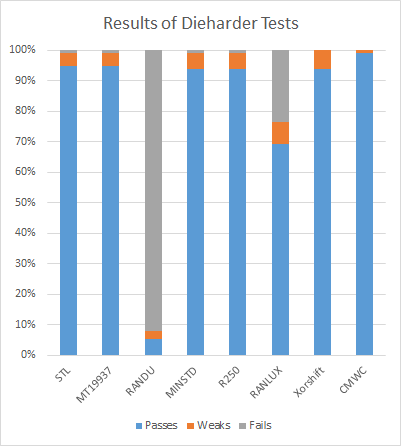
\includegraphics[width=\linewidth]{figures/passesweaksfails.png}
    \end{center}
    \caption{Percentage bar graph of results of Dieharder test results for implemented RNGS.}
    \label{fig:passesweaksfails}
\end{figure}

% http://www.tablesgenerator.com/
\begin{table}[tb]
    \caption{Table displaying Dieharder results for the implemented RNGs.}
    \label{tab:speed}
    \begin{center}
        \begin{tabular}{l|ccc}
        \hline
        \hline
\textbf{RNG Name} & \textbf{Passes} & \textbf{Weaks} & \textbf{Fails} \\
        \hline
STL               & 108             & 5              & 1              \\
MT19937           & 108             & 5              & 1              \\
RANDU             & 6               & 3              & 105            \\
MINSTD            & 107             & 6              & 1              \\
R250              & 107             & 6              & 1              \\
RANLUX            & 79              & 8              & 27             \\
Xorshift          & 107             & 7              & 0              \\
CMWC              & 113             & 1              & 0 \\
        \hline
        \hline
        \end{tabular}
    \end{center}
\end{table}


Another metric worth measuring is RNG speed. This metric has been alluded in Section~\ref{sec:classes}, but is formally measured in random numbers per second. Luckily, Dieharder measures this metric already. As expected, the STL implementation of the Mersenne Twister is quite fast (as is much of the STL), and the RANLUX implementation is slow (because it must discard so many numbers to keep the quality of output high). Of the other RNGs, our Mersenne Twister is the most complicated, and as a result it is the slowest. RANDU is simple and fast, and the other algorithms hover around the same speed. The data is presented graphically in Figure~\ref{fig:speed} and tabularly in Table~\ref{tab:speed}. These speeds were measured on a laptop with an Intel Core i7-4600U CPU @ 2.10GHz with 4 cores.

It is important to remember that these speeds must be considered to be relative. These RNGs must be piped through the shell, as opposed to the GNU Scientific Library RNGs built into the Dieharder binary, and as a result, they can be passed to Dieharder faster.

\begin{figure}[tb]
    \begin{center}
        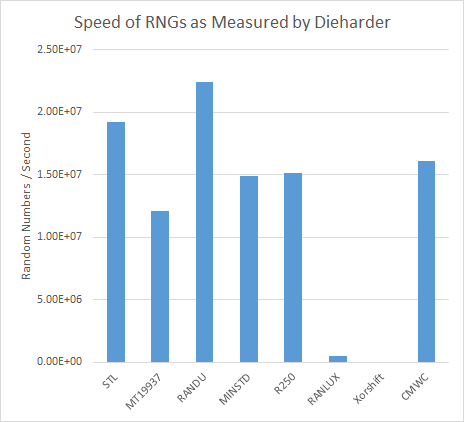
\includegraphics[width=\linewidth]{figures/speed.png}
    \end{center}
    \caption{Speed of implemented RNGs in random numbers per second as measured by Dieharder.}
    \label{fig:speed}
\end{figure}

% http://www.tablesgenerator.com/
\begin{table}[tb]
    \caption{Table displaying speeds of implemented RNGs as measured by Dieharder.}
    \label{tab:passesweaksfails}
    \begin{center}
        \begin{tabular}{l|c}
        \hline
        \hline
\textbf{RNG Name} & \textbf{Speed} \\
        \hline
STL       &  1.91E+07  \\
MT19937   &  1.26E+07  \\
RANDU     &  2.18E+07  \\
MINSTD    &  1.49E+07  \\
R250      &  1.51E+07  \\
RANLUX    &  5.00E+05  \\
Xorshift  &  7.90E+06  \\
CMWC      &  4.30E+06  \\
TinyMT    &  7.97E+06  \\

        \hline
        \hline
        \end{tabular}
    \end{center}
\end{table}


Finally, a measure that cannot be easily determined empirically, and instead falls under analytical testing, is that of period length. As described in Section~\ref{sec:classes}, as the complexity of the generator goes up, the period also goes up. The Mersenne Twister has a particularly large period several orders of magnitude larger than more simple ones, expect for the particular CMWC generator chosen. Though this generator stores far more state than the standard Mersenne Twister implementation, it is significantly faster and has a period several orders of magnitude greater than the other generators. Period lengths for implemented RNGS are displayed tabularly in Table~\ref{tab:period}.

% http://www.tablesgenerator.com/
\begin{table}[tb]
    \caption{Table of periods of implemented RNGs.}
    \label{tab:period}
    \begin{center}
        \begin{tabular}{l|c}
        \hline
        \hline
\textbf{RNG Name} & \textbf{Period Length} \\
        \hline
STL               & $2^{19937}-1$  \\
MT19937           & $2^{19937}-1$  \\
RANDU             & $2^{29}$       \\
MINSTD            & $2^{31}-1$     \\
R250              & $2^{250}-1$    \\
RANLUX            & $10^{171}$       \\
Xorshift          & $2^{128}-1$    \\
CMWC              & $2^{131104}$   \\
TinyMT            & $2^{127}-1$    \\
        \hline
        \hline
        \end{tabular}
    \end{center}
\end{table}



\section{Conclusion}
\label{sec:conclusion}
We anticipate enjoying this project and look forward to reproducing some interesting PRNGs.


\bibliographystyle{IEEEtran}
\bibliography{IEEEabrv,sections/bibliography}

\end{document}
